\documentclass[12pt]{article}
\usepackage[utf8]{inputenc}
\usepackage[T1]{fontenc} % uses T1 fonts (better quality)
\usepackage{lmodern}
\usepackage[dvipsnames]{xcolor}
\usepackage[margin=2cm]{geometry}
\geometry{top=1.5cm}
\usepackage{graphicx} \graphicspath{ {./Images/} }
\usepackage{pdfpages}
\usepackage{booktabs}   % for table borders
\usepackage{amsmath,bm,amssymb}
\usepackage{mathtools}
\usepackage[makeroom]{cancel}
\usepackage{tikz} \usetikzlibrary{shapes,arrows}
% \usepackage{minted} \usemintedstyle{friendly}
\usepackage{enumitem}
\makeatletter
\renewcommand{\thefigure}{8.\@arabic\c@figure}
\definecolor{CrispBlue}{HTML}{0176AE}
\makeatother

\begin{document}
 	\begin{center}
    \line(1,0){300}\\[0.25cm]
 	\Large{\bfseries ECE540: Homework \#4}\\
 	\textsc{\large David Kirby}\\
 	\textsc{\large Due: 08 November 2020}\\
 	\line(1,0){300}\\[0.75cm]
 	\end{center}
\section*{Chapter 8 (\(\bm{7^{th}}\) Edition)}
\subsection*{Review Questions}
\begin{enumerate}
\subsubsection*{Section 8.1}
\item R1. What are the differences between message confidentiality and message integrity? Can you have confidentiality without integrity? Can you have integrity without confidentiality? Justify your answer.\par
\color{CrispBlue}Confidentiality means that if the intruder intercepts a ciphertext message, they cannot determine the plaintext message. Message integrity means that the receiver can detect if the message was tampered with (plaintext or ciphertext). Yes, it's possible to have confidentiality without integrity (the message could be altered by other means, but the intruder still would not be able to determine the plaintext). Yes, it's possible to have integrity without confidentiality (sending a message as plaintext is an example of this).\color{black}
\vspace{-1em}\subsubsection*{Section 8.2}
\item R3. From a service perspective, what is an important difference between a symmetric-key system and a public-key system?\par
\color{CrispBlue}In a symmetric-key system, both parties share a secret key. In a public-key system there are public and private keys, meaning different encryption and decryption keys.\color{black}
\item R4. Suppose that an intruder has an encrypted message as well as the decrypted version of that message. Can the intruder mount a ciphertext-only attack, a known-plaintext attack, or a chosen-plaintext attack?\par
\color{CrispBlue}A known-plaintext attack since the intruder has both the encrypted and decrypted version of the message.\color{black}
\item R5. Consider an 8-block cipher. How many possible input blocks does this cipher have? How many possible mappings are there? If we view each mapping as a key, then how many possible keys does this cipher have?\par
\color{CrispBlue}\(2^8 \) possible input blocks; \(2^8!\) possible mappings; and \(2^8!\) possible keys.\color{black}
\item R7. Suppose \(n=10,000,\ a=10,023,\ b=10,004\). Use an identity of modular arithmetic to calculate in your head \( (a \cdot b)\bmod{n}\).
\color{CrispBlue}
\begin{align*}
	(a \cdot b)\bmod{n}
	=(a\bmod{n}) \cdot (b\bmod{n})
	=23 \cdot 4
	=92
\end{align*}
\color{black}
\end{enumerate}
\vspace{-3em}
\subsection*{Problems}
\begin{enumerate}
	\item P1. Using the monoalphabetic cipher in Figure 8.3, encode the message “This is an easy problem.” Decode the message “rmij’u uamu xyj.”
	\setcounter{figure}{2}
		\begin{figure}[h!]
		\centering
		\includegraphics[width=0.85\textwidth]{./Images/Fig08-003.png}
		\caption{A monoalphabetic cipher}
		\end{figure}\par
	\color{CrispBlue}Encoded message: \texttt{Uasi si mj cmiw lokngch.}\\
	Decoded message: \texttt{wasn't that fun.}\color{black}
	\item P2. Show that Trudy’s known-plaintext attack, in which she knows the (ciphertext, plaintext) translation pairs for seven letters, reduces the number of possible substitutions to be checked in the example in Section 8.2.1 by approximately \(10^9\).\par
	\color{CrispBlue}Normally, the monoalphabetic ciphertext pairs would be 26!, but with 7 letters known, this brings the pairs to 19!. The difference between them would be \(26\cdot25\cdot24\cdot23\cdot22\cdot21\cdot20\approx10^9\).\color{black}
	\item P9. In this problem, we explore the Diffie-Hellman (DH) public-key encryption algorithm, which allows two entities to agree on a shared key. The DH algorithm makes use of a large prime number \(p\) and another large number \(g\) less than \(p\). Both \(p\) and \(g\) are made public (so that an attacker would know them). In DH, Alice and Bob each independently choose secret keys, \(S_A\) and \(S_B\), respectively. Alice then computes her public key, \(T_A\), by raising \(g\) to \(S_A\) and then taking \(\bmod{\ p}\). Bob similarly computes his own public key \(S_B\) by raising \(g\) to \(S_B\) and then taking \(\bmod{\ p}\). Alice and Bob then exchange their public keys over the Internet. Alice then calculates the shared secret key \(S\) by raising \(T_B\) to \(S_A\) and then taking \(\bmod{\ p}\). Similarly, Bob calculates the shared key \(S'\) by raising \(T_A\) to \(S_B\) and then taking \(\bmod{\ p}\).
		\begin{enumerate}
			\item Prove that, in general, Alice and Bob obtain the same symmetric key, that is, prove \(S=S'\).
			\color{CrispBlue}
			\begin{align*}
				S&=T_B^{S_A}\bmod{p}\\
				&=\left(g^{S_B}\bmod{p}\right)^{S_A}\bmod{p}\\
				&=\left(g^{S_A}\bmod{p}\right)^{S_B}\bmod{p}\\
				&=T_A^{S_B}\bmod{p}\\
				&=S'
			\end{align*}\color{black}\vspace{-1em}
			\item With \(p=11\) and \(g=2\), suppose Alice and Bob choose private keys \(S_A=5\) and \(S_B=12\), respectively. Calculate Alice’s and Bob’s public keys, \(T_A\) and \(T_B\). Show all work.
			\color{CrispBlue}
			\begin{align*}
				T_A&=g^{S_A}\bmod{p}	&T_B&=g^{S_B}\bmod{p}\\
				&=2^5\bmod{11}			&&=2^{12}\bmod{11}\\
				&=10					&&=4
			\end{align*}\color{black}
			\item Following up on part (b), now calculate \(S\) as the shared symmetric key. Show all work.
			\color{CrispBlue}
			\begin{align*}
				S&=T_B^{S_A}\bmod{p}\\
				&=4^{5}\bmod{11}\\
				&=1
			\end{align*}\color{black}\vspace{-1em}
			\item Provide a timing diagram that shows how Diffie-Hellman can be attacked by a man-in-the-middle. The timing diagram should have three vertical lines, one for Alice, one for Bob, and one for the attacker Trudy.
			\color{CrispBlue}\begin{center}
            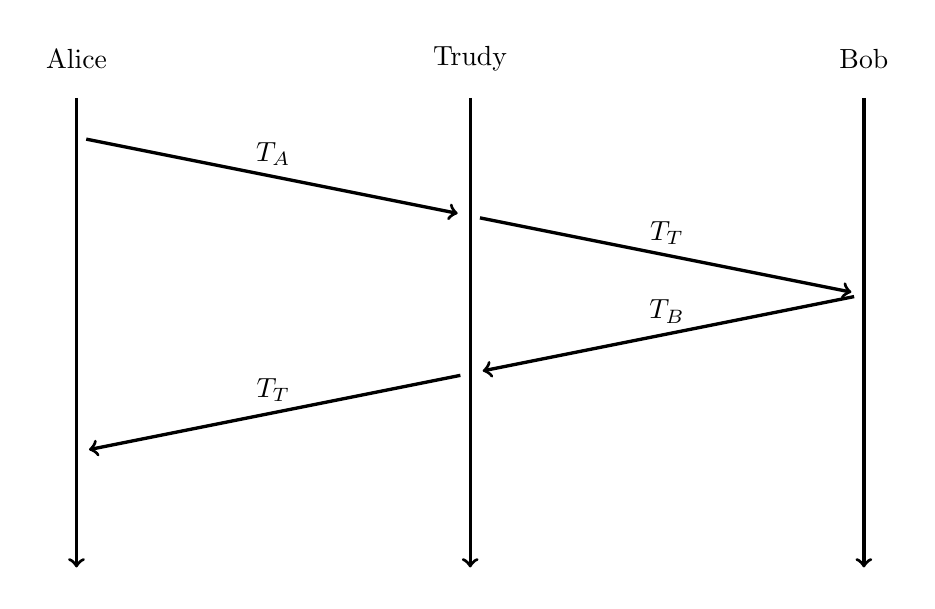
\begin{tikzpicture}[scale=2,shorten >=1pt]
                \matrix[column sep=0cm]{
					\node (Alice) at (0.5,0.5) {$\rm{Alice}$};
					\node (Trudy) at (5.5,0.5) {$\rm{Trudy}$};
					\node (Bob) at (10.5,0.5) {$\rm{Bob}$};
					\node (TA) at (0.5,-0.5) {};
					\node (TT) at (5.5,-1.5) {};
					\node (TB) at (10.5,-2.5) {};
					\node (TA2) at (0.5,-4.5) {};
					\node (TT2) at (5.5,-3.5) {};
					\draw[->][very thick] (0.5,0)--(0.5,-6);
					\draw[->][very thick](5.5,0)--(5.5,-6);
					\draw[->][very thick](10.5,0)--(10.5,-6);

					\path[->][very thick]
					(TA) edge node[above]{$T_A$} (TT)
					(TT) edge node[above]{$T_T$} (TB)
					(TB) edge node[above]{$T_B$} (TT2)
					(TT2) edge node[above]{$T_T$} (TA2);
					\\
                    };
                \end{tikzpicture}
                \\\
            \end{center}Trudy intercepts Alice's public key and sends her own key to Bob instead. When Bob sends his key to Alice, Trudy intercepts that as well, meaning the Trudy can now has both keys and can generate the shared key between Bob and Alice.\color{black}
		\end{enumerate}
	\item P12. Suppose Alice and Bob share two secret keys: an authentication key \(S_1\) and a symmetric encryption key \(S_2\). Augment Figure 8.9 so that both integrity and confidentiality are provided.
	\setcounter{figure}{8}
	\begin{figure}[h!]
	\centering
	\includegraphics[width=0.85\textwidth]{./Images/Fig08-009.png}
	\caption{MAC augmented with symmetric encryption key \(S_2\)}
	\end{figure}\\
	\color{CrispBlue}Please see revised Figure 8.9 above for addition of symmetric encryption key \(S_2\).\color{black}
	\item P15. Consider our authentication protocol in Figure 8.18 in which Alice authenticates herself to Bob, which we saw works well (i.e., we found no flaws in it). Now suppose that while Alice is authenticating herself to Bob, Bob must authenticate himself to Alice. Give a scenario by which Trudy, pretending to be Alice, can now authenticate herself to Bob as Alice. (\textit{Hint}: Consider that the sequence of operations of the protocol, one with Trudy initiating and one with Bob initiating, can be arbitrarily interleaved. Pay particular attention to the fact that both Bob and Alice will use a nonce, and that if care is not taken, the same nonce can be used maliciously.)\par
	\color{CrispBlue}This is similar to modern-day catfishing where an intruder pretends to be someone else. In this case, Trudy initiates contact with Bob by pretending to be Alice; Bob authenticates himself by sending his and Alice's shared key; Trudy cannot reply yet as she does not know the key. Bob sends a nonce, Trudy uses that as her response back to Bob, and Bob essentially authenticates himself using his own key instead of Alice's. This now gives Trudy the nonce shared key. She can now reply back to Bob with this nonce key making Bob think she is Alice.
	\color{black}
	\item P19. Consider the Wireshark output below for a portion of an SSL session.
	\setcounter{figure}{-1}
	\begin{figure}[h!]
	\centering
	\includegraphics[width=0.85\textwidth]{./Images/UnFig08-001.png}
	\caption{(Wireshark screenshot reprinted by permission of the Wireshark Foundation.)}
	\end{figure}
	\begin{enumerate}
		\item Is Wireshark packet 112 sent by the client or server?\par
		\color{CrispBlue}Client
		\color{black}
		\item What is the server’s IP address and port number?\par
		\color{CrispBlue}IP: \texttt{216.75.194.220}\\Port: \texttt{443}
		\color{black}
		\item Assuming no loss and no retransmissions, what will be the sequence number of the next TCP segment sent by the client?\par
		\color{CrispBlue}Sequence \#: 283
		\color{black}
		\item How many SSL records does Wireshark packet 112 contain?\par
		\color{CrispBlue}Packet 112 contains 3 SSL records.
		\color{black}
		\item Does packet 112 contain a Master Secret or an Encrypted Master Secret or neither?\par
		\color{CrispBlue}Packet 112 contains an Encrypted Master Secret.
		\color{black}
		\item Assuming that the handshake type field is 1 byte and each length field is 3 bytes, what are the values of the first and last bytes of the Master Secret (or Encrypted Master Secret)?\par
		\color{CrispBlue}First byte: \texttt{bc}\\ Last byte: \texttt{29}
		\color{black}
		\item The client encrypted handshake message takes into account how many SSL records?\par
		\color{CrispBlue}Client encrypted handshake: 6 SSL records
		\color{black}
		\item The server encrypted handshake message takes into account how many SSL records?\par
		\color{CrispBlue}Server encrypted handshake: 9 SSL records
		\color{black}
	\end{enumerate}
	\item P20. In Section 8.6.1, it is shown that without sequence numbers, Trudy (a woman-in-the middle) can wreak havoc in a TLS session by interchanging TCP segments. Can Trudy do something similar by deleting a TCP segment? What does she need to do to succeed at the deletion attack? What effect will it have?\par
	\color{CrispBlue}Yes, Trudy could achieve the same chaos as without sequence numbers. In order for deleting segments to work, Trudy would need to adjust the sequence numbers accordingly, otherwise Bob and Alice would notice that they did not receive the correct number of segments. If Trudy could accomplish sequence renumbering, Bob and Alice would be receiving a stream with missing packets and never even know it.
	\color{black}
\end{enumerate}
\end{document}